% =============================================================================================
% STANDALONE EXPORT OF §4 FOR EXTERNAL COLD REVIEW.
%
% Contains §4 exactly as it stands in main.tex, together with its two figures. Section, figure
% and equation numbering, cross-references and citations are all live — nothing is re-typed for
% this export, so it cannot drift from the manuscript. The two figure floats live in
% sections/04_figures.tex, which main.tex and this file both \input.
%
% Build:  tectonic -X compile paper/review_s4.tex
% =============================================================================================
\documentclass[10pt]{article}
\usepackage{preprint}

\author{}
\date{}

\begin{document}

% §4 forward-references three things outside this export: §3 and two of its subsections, the
% Limitations section, and Figure 8 (the decision-surface panel, which lives in §6). Bind each
% label to the number it carries in the manuscript so every reference resolves to what a reader
% of the full paper would see.
\makeatletter
\@namedef{r@sec:mechanism}{{3}{1}{Mechanism}{section.3}{}}
\@namedef{r@sec:mechanism@cref}{{[section][3][]3}{1}}
\@namedef{r@sec:mech-fix}{{3.6}{1}{Intervention}{subsection.3.6}{}}
\@namedef{r@sec:mech-fix@cref}{{[subsection][6][3]3.6}{1}}
\@namedef{r@sec:limitations}{{7}{1}{Limitations}{section.7}{}}
\@namedef{r@sec:limitations@cref}{{[section][7][]7}{1}}
\@namedef{r@fig:verdict}{{8}{1}{The decision surface}{figure.8}{}}
\@namedef{r@fig:verdict@cref}{{[figure][8][]8}{1}}
\makeatother

\setcounter{section}{3}   % so §4 numbers as §4, matching the manuscript
\setcounter{figure}{4}    % Figures 1--4 precede this section
\setcounter{equation}{0}
\setcounter{table}{0}

{\centering
{\normalsize\textsc{Section 4 --- export for external review}}\\[0.5em]
{\Large\bfseries Capacity Eviction in Reconstruction-Trained Tokenizers}\\[0.4em]
{\small\color{tolgrey} Draft of \today\ --- section text frozen pending review}\\[1.6em]
}

\noindent\textbf{Note to the reviewer.} This is \S4 of a paper in preparation, exported verbatim
from the manuscript with its two figures. Numbering matches the manuscript: \S4.1--\S4.8,
\cref{eq:netret,eq:cost}, and Figures~5 and~6. \S4 specifies the experiment; it reports no result,
and the pre-registered run has not been executed. References to \S3, \S7 and Figure~8 point
outside this export and are bound to their manuscript numbers.

\medskip
\noindent\textbf{What we would most like challenged.} (i) Whether the five cells, as specified,
can separate microstructure \emph{information} from input \emph{capacity} --- \S4.3 states that
they cannot fully, and quantifies nothing; we would like to know whether the disclosure is
sufficient or whether the design should not ship without the sixth cell. (ii) Whether the
execution filter and its selection procedure (\S4.4) are sound given that the filter never bound
on the calibration fixture. (iii) Whether the decision rule (\S4.6) is genuinely falsifiable ---
whether there is a result we would be forced to call a null. (iv) Whether the multiple-testing and
power treatment (\S4.7) is honest about what five seeds can and cannot resolve. (v) Any number
that does not follow from what is stated.

\bigskip
\hrule
\bigskip

% =============================================================================================
% §4 Experimental design. Zero run dependency: the design is frozen and every value below is a
% pin or a measurement that already exists. Artifact citations in % comments; strip before final.
% =============================================================================================
\section{Experimental design}
\label{sec:setup}

The mechanism of \cref{sec:mechanism} says that a reconstruction-trained tokenizer will evict
microstructure unless it is built not to. This section describes the experiment that asks the
separate question the paper is organized around: whether real trade-flow imbalance, carried through
a tokenizer built to preserve it, survives to a cost-aware trading decision. The design was frozen
before any of its numbers existed, and this section describes it as frozen.

\subsection{Five cells}
\label{sec:cells}

The experiment is a $2\times2$ over the two factors that could plausibly explain a difference ---
the quantizer and the input arm --- plus a fifth cell that isolates the one thing a $2\times2$
cannot: whether an effect attributed to microstructure is really microstructure.
\Cref{fig:design} shows the layout; the registry that the runner reads is the authority.
% artifact: src/trikaal/train/cells.py:40-44 — CellSpec(1,'bsq',ARM_OHLCV), (2,'fsq',ARM_OHLCV), (3,'bsq',ARM_MICRO), (4,'fsq',ARM_MICRO), (5,'fsq',ARM_MICRO_SHUFFLED)

Cells 1 and 2 receive the seven OHLC-shape, volume and amount dimensions only; cells 3 and 4
additionally receive the six microstructure dimensions (indices 7--12: trade-flow imbalance,
signed count imbalance, trade count, mean trade size, trade-size dispersion, large-trade share).
Cells 1 and 3 quantize with binary spherical quantization; cells 2 and 4 with finite scalar
quantization. Cell 5 is cell 4 with the microstructure block shuffled, and is the placebo.
% artifact: src/trikaal/constants.py :: OHLCV_ONLY_IDX = (0..6), MICRO_DIMS_IDX = (7..12), FEATURE_NAMES

The comparison that carries the paper is the paired difference $\Delta\IR(4-5)$. The others are
support: $\IR(4)-\IR(2)$ asks whether the microstructure arm beats the OHLCV arm without reference
to the placebo, and the two BSQ cells anchor the quantizer axis. We are explicit in
\cref{sec:limitations} that the three marginals involving a BSQ arm are withdrawn as claims,
because the BSQ implementation has no external reference point; they are reported, not claimed.

In the OHLCV-only arm the six microstructure dimensions are \emph{removed} from the input rather
than supplied and left uninformative, so that arm's feature width is seven rather than sixteen.
That choice matters for interpreting the legibility gate, which is undefined for an arm with no
microstructure channel and is exempted there by a named registry entry rather than by silence.
% src: src/trikaal/train/arms.py:49-59 — ARM_OHLCV: False with an explicit exemption reason string

\subsection{Capacity is controlled, not assumed}
\label{sec:parity}

A comparison between two quantizers is meaningless if one of them simply has more room. We
therefore control the two quantities that determine room, and report both rather than asserting
parity. The finite-scalar arm uses per-dimension levels $(11,9,9,7,7,5,5)$, split into a coarse
subtoken of $891$ codes and a fine subtoken of $1225$, for $20.058$ bits per bar; the
binary-spherical arm spends $10+10$ bits for $20.000$. The two differ by $0.058$ bits per bar,
inside a pre-registered parity band of $19.5$--$20.5$.
% artifact: runs_manifest/m6_interface_respec_design_pass.json :: g_parity_new_layout.{bpt_a=20.05784765541185, bpt_b=20.0}; src/trikaal/constants.py :: FSQ_BPT_BAND=(19.5,20.5)

The predictor realizes $31{,}795{,}200$ parameters at the finite-scalar vocabulary and
$31{,}725{,}568$ at the binary-spherical one. Of each, $10{,}493{,}952$ --- a third of the model
--- are the multi-token-prediction heads, which are trained and shipped; the backbone excluding
them is $21{,}301{,}248$ and $21{,}231{,}616$ respectively, and that is the figure the
construction gate pins. We quote both, and quote the total first, because the released weights
make the total checkable in one line and a reader who computes it should find our number. The two
arms differ by $69{,}632$ parameters --- $0.219\%$ of the realized model, equivalently $0.327\%$
of the backbone --- arising entirely from vocabulary-dependent embedding and output-head rows.
The heads are identical in both arms at $10{,}493{,}952$ each, so the gap is the same absolute
quantity on either basis. The backbone
is otherwise identical across all five cells: eight layers, model width $512$, feed-forward width
$1024$, eight heads, and a context of $512$ bars. It is held fixed on purpose. The tokenizer is
the object under study; the backbone is the instrument that measures it.
% artifact: THE COUNTS ARE CITED TO WHAT A READER CAN RECOMPUTE, not to an instruction document.
%   BSQ arm (the released weights): runs_manifest/m6_weights_release.json ::
%     units.{0,2,4}.predictor_parameter_groups.{n_params_realized_total = 31725568,
%     n_params_mtp = 10493952, backbone = 21231616}, and .how_to_verify prints the recipe --
%     "load predictor.pt and sum numel() over state_dict to reproduce n_params_realized_total".
%   FSQ arm: the released manifest does NOT carry 31,795,200, because the shipped units are cell 1
%     (BSQ). That figure is summed from runs_cloud/ckpt_cell4_seed0/predictor.pt and is asserted
%     at render time by paper/figures/make_fig5_design.py::_verify_params(), which raises on a
%     wrong constant and has been observed to do so.
%   The engineering-norms file remains the authority for the NORMS it states; it is not cited for
%   a measured quantity, because an instruction document ASSERTS a number where a manifest lets a
%   reader VERIFY one. Percentages computed here.

Every cell trains under the same budget: $26{,}003$ steps at batch $32$ and context $512$, on the
same draw. That budget is matched and fixed rather than chosen per cell by early stopping. The
alternative --- stopping each cell when its own validation loss saturates --- would give five
different budgets and confound $\Delta\IR(4-5)$ with ``cell 4 trained longer'', which is the same
class of confound the placebo exists to remove. The cost is that no cell is guaranteed to be at
its own optimum; saturation is measured and reported rather than optimized against.
% artifact: runs_manifest/m6_training_budget.json; docs/m6_design.md:18 (all cells share the training draw)

\subsection{The placebo, and the handicap it creates}
\label{sec:setup-placebo}
\label{sec:placebo}

The placebo answers a question no capacity control can: whether an effect attributed to
microstructure comes from microstructure's \emph{information} or merely from the model having six
more input channels to spend capacity on. Cell 5 receives the same six channels, with the same
marginal distributions, carrying no usable information.

The shuffle permutes the six microstructure dimensions as a block, within each contiguous segment
of a symbol, with a full within-segment permutation rather than a fixed block length. Three
properties are enforced rather than assumed. The block moves as a unit, so within-bar structure
\emph{among} the microstructure dimensions survives and only their relationship to everything else
is destroyed. The mask travels with the value, because permuting values alone would strand fill
values on valid bars and real values on masked ones --- a defect found in review and fixed before
any training. And the permutation is derived from the run seed and the symbol together, so the
train and evaluation paths shuffle identically.
% src: src/trikaal/eval/placebo.py — block permutation, cell5_seed(seed, symbol) = (seed << 16) ^ crc32(symbol)
% artifact: docs/BUILD_RECORD.md D6 — the (value, mask) pairing defect, closed 2cac96f

\Cref{fig:design} reports what the shuffle measurably does. It destroys the contemporaneous link
between microstructure and price shape, from mean absolute correlation $0.2037$ to $0.0005$, and
it destroys microstructure's own lag-1 autocorrelation, from $0.4165$ to $0.0006$. It leaves the
within-block correlation at $0.2886$ and the within-OHLCV correlation at $0.3105$, both unchanged.
% artifact: docs/m6_c12_placebo_mechanism.md — the four-row before/after table

This is where the design's principal known weakness lives, and we state it rather than let a
reader find it. Because cell 4's microstructure dimensions are correlated with price at $0.20$ and
autocorrelated at $0.42$, part of the capacity they consume is \emph{amortized} against structure
the code is already carrying. Shuffling removes that amortization along with the information, so
cell 5 pays a capacity price cell 4 does not. The consequence is a forfeit stated in the
pre-registered rule string itself: $\Delta\IR(4-5)$ is (information) $+$ (capacity handicap), and
the paper does not claim the information effect alone clears any threshold.
% artifact: src/trikaal/eval/verdict.py — clause 4 rule string names the composite quantity explicitly
The handicap is not quantified in information-ratio units, and \cref{sec:limitations} carries that
as an open disclosure rather than a resolved question.

\subsection{The headline metric, the geometry, and the decision rule}
\label{sec:metric}
\label{sec:geometry}
\label{sec:decision}

The headline is a cost-aware net information ratio, annualized, computed on a portfolio return
series. For a position of sign $s$ opened at the close of bar $t+1$ and closed $h$ bars later, the
realized net log-return subtracts execution and funding cost directly:
\begin{equation}
  r^{\text{net}} \;=\; s \log\!\frac{C_{t+h}}{C_{t+1}} \;-\; c_{\text{total}} \;-\; c_{\text{funding}},
  \qquad c_{\text{total}} = 2\,c_{\text{side}} .
  \label{eq:netret}
\end{equation}
A position is taken only where the forecast magnitude exceeds a threshold proportional to cost,
$\theta = \kappa c$, so the metric never rewards a forecast too small to pay for its own execution.
Entry at $t+1$'s close, not $t$'s, is the causal-safety margin: a decision made on bar $t$ cannot
transact at a price inside bar $t$. Information coefficient, rank information coefficient, mean
absolute error and $R^2$ are reported as diagnostics and none of them decides anything.
% artifact: src/trikaal/eval/harness.py — per-position net return; entry at t+1 close, exit at t+h;
%   theta = kappa * c_modeled per src/trikaal/eval/xsection.py:335.

Evaluation is purged walk-forward with an embargo, never a random split. The training region is
used once and never refitted; five forward blocks carry the headline; a $120$-bar embargo separates
each training window from the labels it must not see, built as the $60$-bar label look-forward plus
a $60$-bar serial-correlation margin. \Cref{sec:lim-embargo} reports the measurement that premise
rests on, including the channel where it does not hold.

\textbf{The decision rule was written, timestamped and committed before any cell was trained}, and
it is conjunctive: the primary outcome is \textsc{survives} only if none of five clauses fails, and
\textsc{null} otherwise. The clauses require, in order, that the one-sided $95\%$ lower bound of
$\Delta\IR(4-5)$ exceeds zero; that the effect reaches the paired minimum detectable effect, so an
effect too small for this design to resolve cannot be reported as one; that the lower bound of
$\IR(4)-\IR(2)$ exceeds zero, a comparison not involving the placebo at all, so a placebo pathology
cannot by itself produce a positive verdict; that $\Delta\IR(4-5)$ reaches an economic floor of
$0.5$ fixed before data, with the rule string naming the tested quantity as information plus
capacity handicap so the manifest cannot be read as claiming the information effect alone; and that
the deflated Sharpe ratio is at least $0.95$ over the enumerated trial set. \label{tab:verdict}
Two guards sit outside the clauses and are halt-only --- they can refuse to report an outcome their
inputs cannot support, and can never turn \textsc{survives} into \textsc{null} or the reverse.
\Cref{app:repro} gives the pinned constants, the exact clause strings, the trial enumeration, the
minimum-detectable-effect derivation and the guards' asymmetries; they are machinery, and a reader
does not need them to follow the result.
% artifact: src/trikaal/eval/verdict.py — clause keys 1_paired_ci, 2_mde_paired, 3_placebo_validity,
%   4_economic_floor, 5_dsr; ECON_FLOOR_IR = 0.5 defined :74, read :1074.

\textbf{The design's own arithmetic said the likely outcome was negative, and we recorded that
before running it.} The minimum detectable effect at the pinned horizon is $3.518$ annualized
information ratio; our prior for a univariate microstructure signal at that horizon is a rank
information coefficient of $0.0197$. On these numbers, \textsc{null} or \textsc{inconclusive} is
the most likely honest outcome, and \cref{sec:lim-power} states what that costs the design.

\subsection{Pre-registration as the integrity mechanism}
\label{sec:prereg}

Everything above --- the cells, the parity band, the placebo construction, the five clauses and
their thresholds, the horizon, the cost, the $\kappa$ grid, the seed count, the trial count and the
null basis --- is pinned on a conformance surface that the runner checks before it trains
anything, and each pin carries a mutation test proving the gate rejects its predecessor value.
Changing a pin is not a code edit that a reviewer must catch; it fails the run.
% artifact: src/trikaal/eval/conformance.py; per-pin mutation KATs

The pre-registration is a dated document with an append-only amendment log. Every amendment
records what changed, when, why, and --- where the direction was knowable --- whether it made the
bar easier or harder, recorded before the data that would reveal which. Amendments made after
seeing calibration results are marked as such, including the one described in
\cref{sec:mech-fix}. The log also contains withdrawn claims: statements this project made and
later retracted, retained rather than deleted. We regard that as the load-bearing part. A
pre-registration that only ever records successful predictions is not evidence of discipline; one
that records its own corrections is.
% artifact: docs/m6_prereg.md §7 — amendment log, entries v1.1 through v1.6.27, each dated

% The two figures belonging to §4. Held in their own file so that main.tex and review_s4.tex
% share one copy and the export cannot drift from the manuscript.
\begin{figure}[t]
  \centering
  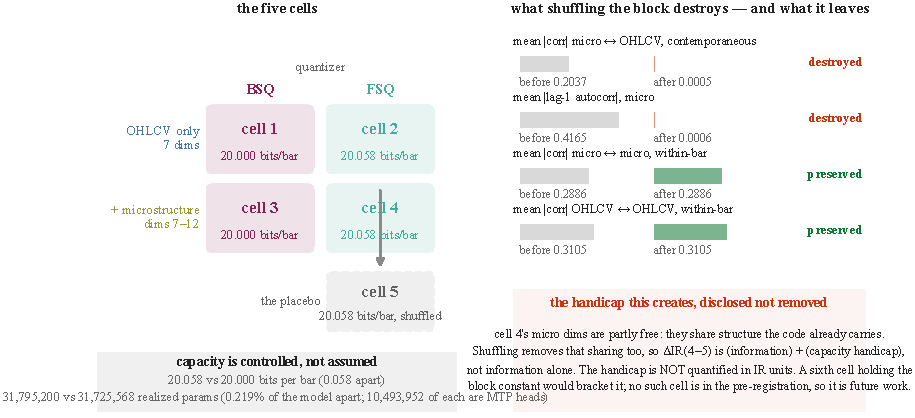
\includegraphics[width=\textwidth]{figures/fig5_design.pdf}
  \caption{\textbf{The five cells, at matched capacity, and the exact reach of the placebo.}
  \emph{Left:} a $2\times2$ over quantizer and input arm, plus a fifth cell that is cell 4 with the
  microstructure block shuffled. Capacity is controlled rather than assumed: the two quantizer arms
  differ by $0.058$ bits per bar and by $0.327\%$ of backbone parameters, so a difference between
  them cannot be attributed to one arm simply having more room. \emph{Right:} what the shuffle
  actually does, measured. It destroys the two things it was built to destroy --- microstructure's
  contemporaneous link to price ($0.2037 \rightarrow 0.0005$) and its own lag-1 autocorrelation
  ($0.4165 \rightarrow 0.0006$) --- and leaves the within-block and within-OHLCV correlations
  exactly as they were. The consequence is stated rather than hidden: because cell 4's
  microstructure dimensions are partly amortized against structure the code already carries,
  shuffling removes that sharing too, so $\Delta$IR(4$-$5) is (information) $+$ (capacity
  handicap). The handicap is not quantified in
  information-ratio units. A sixth cell holding the block constant would bracket it, but no such
  cell appears anywhere in the pre-registration, so it is future work rather than a committed
  contingency, and \cref{sec:limitations} carries the handicap as an open disclosure.}
  \label{fig:design}
\end{figure}
\clearpage
\begin{figure}[t]
  \centering
  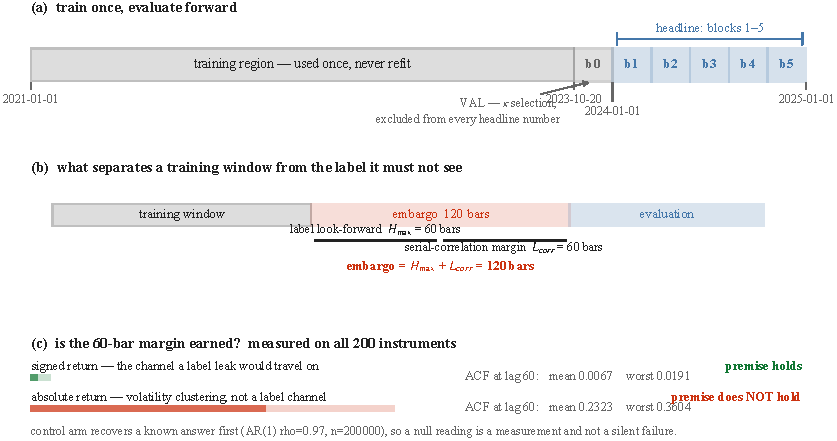
\includegraphics[width=\textwidth]{figures/fig6_validation.pdf}
  \caption{\textbf{Train once, evaluate forward, and pay for the separation.} \textbf{(a)} The training
  region ends at one boundary and is never refit. The forward region is cut into six blocks; block
  0 is spent selecting the execution filter and is excluded from every headline number, so the
  headline is scored on five blocks the selection never saw. \textbf{(b)} Between a training window
  and any label that could contaminate it sit a $60$-bar label look-forward and a $60$-bar
  serial-correlation margin, giving a $120$-bar embargo. \textbf{(c)} The premise behind that
  margin is measured on all $200$ instruments rather than assumed, and a control arm recovers a
  known AR(1) answer first, so a null reading is a measurement and not a silent failure. It holds
  for signed returns --- the channel a label leak would travel on --- at ACF $0.0067$ mean and
  $0.0191$ worst-symbol at lag $60$. It does \emph{not} hold for absolute returns
  ($0.2323$ mean, $0.3604$ worst), which is volatility clustering rather than a label channel;
  \cref{sec:limitations} carries that caveat.}
  \label{fig:validation}
\end{figure}


\clearpage
\bibliographystyle{plainnat}
\bibliography{refs}

\end{document}
